\documentclass[12pt,letterpaper]{article}

% just for the example
\usepackage{lipsum}
% Set margins to 1.5in
\usepackage[margin=1.5in]{geometry}

% for graphics
\usepackage{graphicx}
\graphicspath{{./figures/m1/}}

% for crimson text
\usepackage{crimson}
\usepackage[T1]{fontenc}

% setup parameter indentation
\setlength{\parindent}{0pt}
\setlength{\parskip}{6pt}

% for 1.15 spacing between text
\renewcommand{\baselinestretch}{1.15}

% For defining spacing between headers
\usepackage{titlesec}
% Level 1
\titleformat{\section}
  {\normalfont\fontsize{18}{0}\bfseries}{\thesection}{1em}{}
% Level 2
\titleformat{\subsection}
  {\normalfont\fontsize{14}{0}\bfseries}{\thesection}{1em}{}
% Level 3
\titleformat{\subsubsection}
  {\normalfont\fontsize{12}{0}\bfseries}{\thesection}{1em}{}
% Level 4
\titleformat{\paragraph}
  {\normalfont\fontsize{12}{0}\bfseries\itshape}{\theparagraph}{1em}{}
% Level 5
\titleformat{\subparagraph}
  {\normalfont\fontsize{12}{0}\itshape}{\theparagraph}{1em}{}
% Level 6
\makeatletter
\newcounter{subsubparagraph}[subparagraph]
\renewcommand\thesubsubparagraph{%
  \thesubparagraph.\@arabic\c@subsubparagraph}
\newcommand\subsubparagraph{%
  \@startsection{subsubparagraph}    % counter
    {6}                              % level
    {\parindent}                     % indent
    {12pt} % beforeskip
    {6pt}                           % afterskip
    {\normalfont\fontsize{12}{0}}}
\newcommand\l@subsubparagraph{\@dottedtocline{6}{10em}{5em}}
\newcommand{\subsubparagraphmark}[1]{}
\makeatother
\titlespacing*{\section}{0pt}{12pt}{6pt}
\titlespacing*{\subsection}{0pt}{12pt}{6pt}
\titlespacing*{\subsubsection}{0pt}{12pt}{6pt}
\titlespacing*{\paragraph}{0pt}{12pt}{6pt}
\titlespacing*{\subparagraph}{0pt}{12pt}{6pt}
\titlespacing*{\subsubparagraph}{0pt}{12pt}{6pt}

% Set caption to correct size and location
\usepackage[tableposition=top, figureposition=bottom, font=footnotesize, labelfont=bf]{caption}

% set page number location
\usepackage{fancyhdr}
\fancyhf{} % clear all header and footers
\renewcommand{\headrulewidth}{0pt} % remove the header rule
\rhead{\thepage}
\pagestyle{fancy}

% Overwrite Title
\makeatletter
\renewcommand{\maketitle}{\bgroup
   \begin{center}
   \textbf{{\fontsize{18pt}{20}\selectfont \@title}}\\
   \vspace{10pt}
   {\fontsize{12pt}{0}\selectfont \@author} 
   \end{center}
}
\makeatother

% Used for Tables and Figures
\usepackage{float}

% For using lists
\usepackage{enumitem}

% For using APA Citation format
\usepackage{apacite}

% Custom Quote
\newenvironment{myquote}[1]%
  {\list{}{\leftmargin=#1\rightmargin=#1}\item[]}%
  {\endlist}
  
% Create Abstract 
\renewenvironment{abstract}
{\vspace*{-.5in}\fontsize{12pt}{12}\begin{myquote}{.5in}
\noindent \par{\bfseries \abstractname.}}
{\medskip\noindent
\end{myquote}
}

\begin{document}

% Set Title, Author, and email
\title{Assignment M1}
\author{Snejana Shegheva \\ sshegheva3@gatech.edu}

\maketitle
\thispagestyle{fancy}

\begin{abstract}
Mapping data from one form to another for its ease-of-use is at the core of the \textit{Extract, Transform and Load} process. There exist many tools that can accomplish the task of creating and maintaining a data warehouse. However, sometimes it is advantageous to have a custom solution that allows a user to interact with the data directly during some or all of the ETL phases. In this project, we analyze an internal interface of a \textit{transform} task that prepares the data for use in a personalized recommendation system powered by Artificial Intelligence engines. 
\end{abstract}

\subsection*{Problem Space}
The data ingestion is described by the \textit{Extract, Transform and Load} (ETL) process - a cycle that converts a raw data into structured records more convenient for further Data Analysis and/or uses for Machine Learning algorithms \cite{wiki:etl}. Figure~\ref{fig::1} shows the ETL process from the Source to the Destination. The entire cycle may be completely hidden from the user (full automation of data ingestion), or a human is required to guide the components of the process to reach their desired goal. In this project we focus on the \textit{transform} task that is centered around interactions with the user to alter the original data to meet their needs. For example, a user who looks at the weather feed in Fahrenheit may choose to convert it to Celsius. 

\begin{figure}[H]
\centering
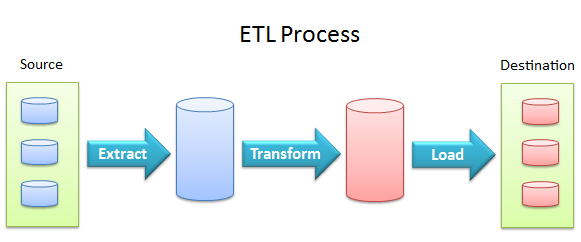
\includegraphics[width=3in, scale=.3]{ETLProcess.png}
\caption{Extract-Transform-Load Process from Data Science Central blogpost on Open Source ETL tools (https://www.datasciencecentral.com/profiles/blogs/10-open-source-etl-tools)}
\label{fig::1}
\end{figure}

To accomplish the data transformation task, a user needs access to the original data, as well as an arsenal of mapping tools suitable to the domain. Figure~\ref{fig::2} shows an existing version of an internal interface \footnote{A very rough version of a custom tool to perform user-driven ETL process.} that we will be analyzing and re-designing to improve user experience in undertaking the transformation task. 

\begin{figure}[H]
\centering
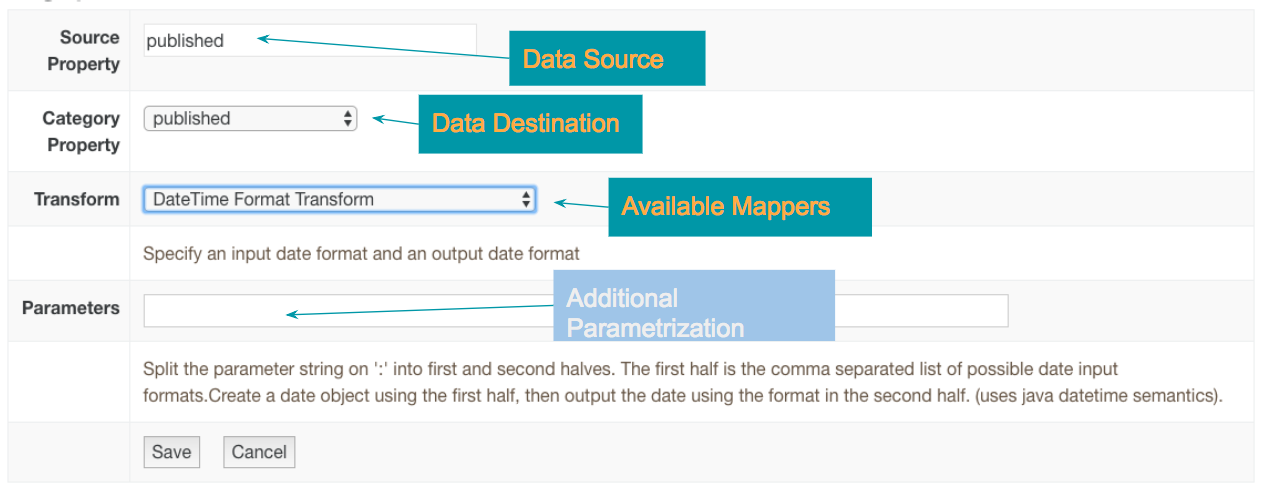
\includegraphics[width=4in, scale=.4]{NaraTransform.png}
\caption{A version of an internal interface for transforming a single data field. Here, the data source is the data from the Arxiv Library collected via ATOM API. User selects the original field, here the \textit{published} date, and wishes to transform it to a different date format.}
\label{fig::2}
\end{figure}

Our main goal is to assess all the weak areas of the existing interface in order to provide recommendations for alternative models that simplify the user interaction without assuming any pre-existing knowledge of the tool.

\subsection*{User Types}
Let's outline the user who is expected to engage in the data transformation task described above. The target user's expertise ranges from a novice (an external business client without extensive technical background) to an expert (data analyst interacting with the tool on a daily basis). The task assumes a basic proficiency with computer interfaces, which is a reasonable assumption given that the expected audience are professionals that use data to make business decisions. The task for different categories of users remains the same; however, the approach for accomplishing it may differ significantly. On the one hand, a user with substantial knowledge of the data (a domain expert) may want to explore complex relationships between the existing variables and generate new outcomes that capture the essence of the observed relationship. On the other hand, a user tasked with a data cleanup process, might not wish to delve into data intricacies, and instead focus on the common exercise of standardizing the content (for example, change a \textit{thousands} separator in the numerical data). 

A context of the task varies significantly and is mainly data-driven. A system for recommending movies involves data on user preferences and feedback. A method for optimizing financial portfolios streams data from financial markets and/or other sources. Therefore, an interface for accomplishing the described goals should be domain agnostic, and abstract the functionality of the transformation process to support a plethora of contexts. In general, a user needs access to a Web interface that allows uploading a data from many sources, and subsequently either loading it to a warehouse as is, or applying necessary and desired transformations to alter the original form. In order to accomplish a transformation task, users need to 1) know \textit{what} data and in what form is currently available, 2) define the rules to \textit{convert} the data from the original to the desired form, 3) \textit{see} the final result to confirm the success, or \textit{receive a feedback} for required adjustments in failure cases. The vast bulk of the user interaction with the interface is expected around the sub-task of defining a transformation rule. Therefore, a good design should focus on simplifying this step by providing an intuitive interface for data manipulation.


\subsection*{Needfinding Plan 1 - Hacks and Workarounds}
We have briefly described what the user's ultimate goal is, and how that can be broken down into sub-goals. In this section, we are going to further zoom into the user's actions for performing the task of data transformation. As our objective is to understand the weaknesses of the existing interface, as shown in Figure~\ref{fig::2}, we analyze the cases where the user breaks out of the provided interface and resorts to various hacks and workarounds to accomplish the task. A user in a Data Scientist role has a frequent need for manipulating the raw data that moves through the ETL pipeline. The main reasons why the user in that role currently changes their intended workflow and performs a subset of the actions outside of the given interface can be summarized by the following three categories: 

\begin{enumerate}
    \item \textbf{Limited functionality}. Before deciding on the transformation rules, a user needs to have a visibility on the data being transformed. In the current interface (see Figure~\ref{fig::3}), user selects the targeted data field, for example a \textit{published date}, and is given an \textit{edit} button. However, the interface does not provide enough information to make a fully informed action on the required transformation rule. Therefore, a workaround\#1:  
    \textit{Load the data in the external interface (command line, Jupyter notebooks, database queries) to explore descriptive statistics of the original field - the most frequent values,  the extreme values, the rate is missing fields, etc.}
    
    \begin{figure}[h]
    \centering
    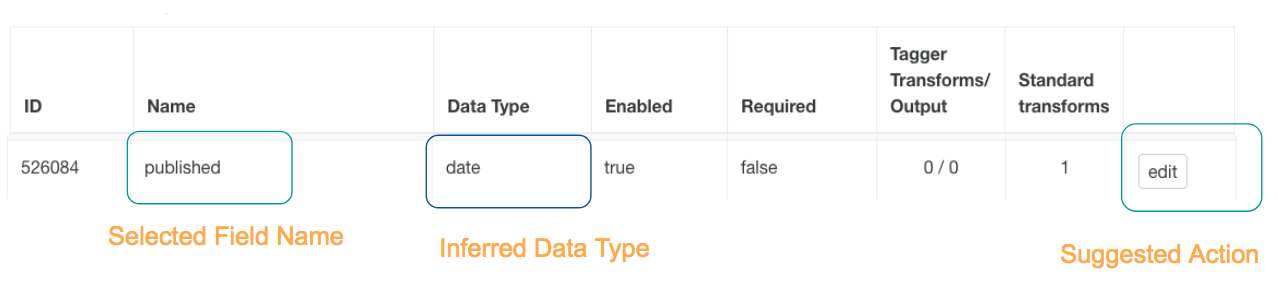
\includegraphics[width=4in, scale=.4]{DataVisibility.png}
    \caption{An example of the interface limitation to provide the user with knowledge of the present data form to enable an informed action.}
    \label{fig::3}
    \end{figure}
    
    
    \item \textbf{Poor Feature Organization}. After the user has decided on the transformation rule, the next step is to map their intentions to one of the of existing transformers. Figure~\ref{fig::4} shows that in the current interfaces the selection is given without consideration for priority or relevance of the transformation to the field being examined. Therefore, a workaround\#2:
    \textit{Browse through previously made transformations (if available) for examples and common use cases, ask colleagues for a bit of advice, or make educated guesses until the right transformer is found}
    
    \begin{figure}[h]
    \centering
    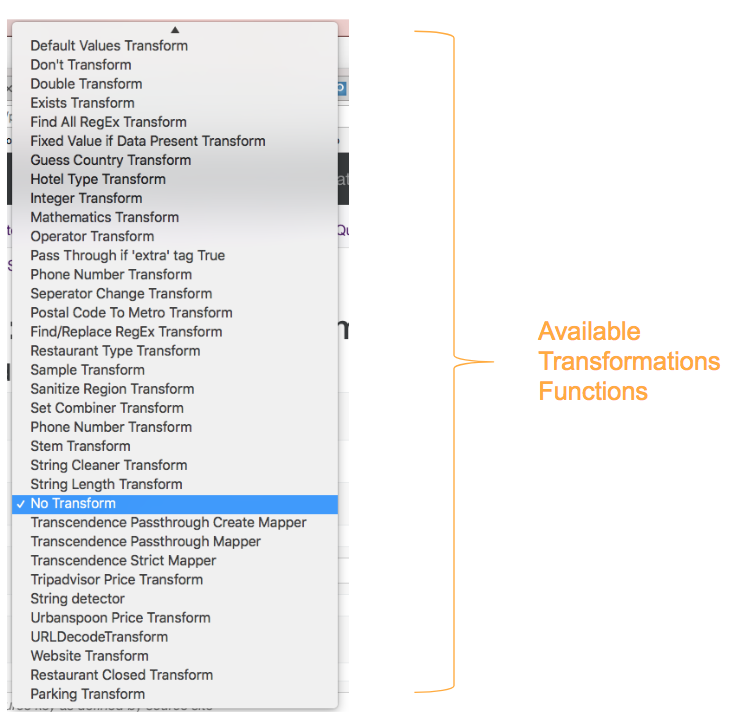
\includegraphics[width=4in, scale=.3]{Transformers.png}
    \caption{An example of the interface that displays ALL available transformation functions without priority or relevance consideration.}
    \label{fig::4}
    \end{figure}
    
    \item \textbf{Bugs in the existing functionality}. Unintended behavior in software happens all the time. The interface needs to provide accessible means to recover from a mistake by undoing an erroneous operation. A user should be comfortable exploring the interface without the fear of irreversibly corrupting the data. A good interface, therefore, should be able to guide the user from the failed state. As the current interface does not provide visibility on the original or the final data (after the applied transformation), there are no means to undo an action where transformation has the unintended effect. Workaround\#3: \textit{Modify the data via direct database access from, hopefully existing, backups.} 
    
\end{enumerate}

The need-finding approach covered in this section connects the user's goals of altering a data feed to the sub-tasks of viewing the existing data, planning the transformation, and confirming the outcome. The approach of need-finding via analysis of hacks and workarounds is susceptible to \textit{observational selection bias} as we tend to notice workarounds when they impact us directly. To avoid this bias, we pair up this approach with another method that seeks to understand the pain points of a larger group of users, preferably with diverse roles.

\subsection*{Needfinding Plan 2 - Errors}
To better understand the user's struggles with the interface, it is useful to analyze the frequencies of two kinds of errors, such as \textit{slips} and \textit{mistakes}. A mental model is a process that explains how a user is thinking about the task regarding actions and outcomes \cite{wiki:mental_model}. When a mental model matches the logic implemented by an algorithm, the user has a correct understanding of the system's functionality. In this case, the user's error can be classified as a slip vs. a mistake where the user has a wrong mental model. The approach for need-finding that focuses on error analysis broadens the spectrum of users in terms of their expertise in the given task. A novice in the field can be guided through the process of transformation by automatically matching the compatible functions to the field subjected to alterations. 

Figure~\ref{fig::5} exemplifies a hypothetical scenario where the user does not have a correct representation of the state and appropriate actions. In this example, the user attempts to transform a field that captures a person's name (\textit{author}) by applying a function that is designed to manipulate \textit{dates}. This is an incompatible operation that should not be allowed by the interface. The analysis of errors for such type outlines a \textit{need} for system's intelligence to understand the input data types and the \textit{schemata} of the available transform to reduce the space of possible matches. An improvement like can decrease the chances for user to apply incorrect action for the task at hand.   

\begin{figure}[h]
\centering
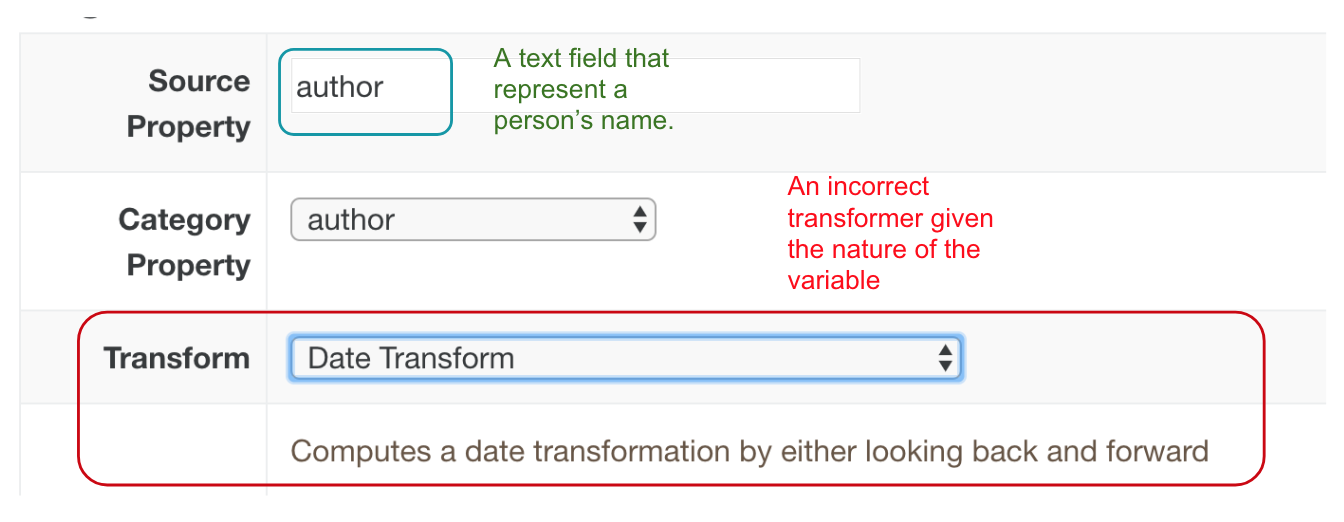
\includegraphics[width=4in, scale=.3]{mistake.png}
\caption{An example of the incorrect user action where their mental model of the underlying process is incorrect. A textual field, such as person's name cannot be computed as a date transformation.}
\label{fig::5}
\end{figure}

When a user has a correct mental model, but still makes an error due to a rushed behavior, there is an opportunity to improve the interface to reduce the chance of \textit{slippage} by altering the nature of interactions. Figure~\ref{fig::6} shows an interface that expects the user to submit a list of characters for String Cleaning. This form of interaction allows easy creation of a typo that can be avoided by modifying the underlying interaction. A change like an abstraction of special characters into a class of invalid characters for a \textit{name} field can improve users' efficiency in performing a transformation task.

\begin{figure}[h]
\centering
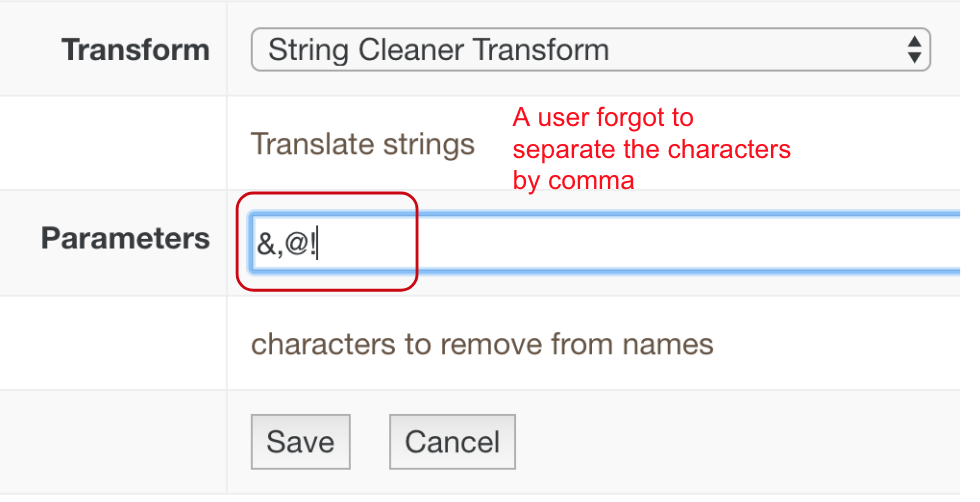
\includegraphics[width=4in, scale=.3]{slip.png}
\caption{An example of the incorrect user action where their mental model of the underlying process is correct, but user can still easily make a mistake by making a typo.}
\label{fig::6}
\end{figure}

Similarly to the approach of Hacks and Workaround, the Error analysis approach is susceptible to the \textit{observational selection} bias. In both methods, the effect of the bias can be reduced by quantitatively measuring the impact those errors have on the productivity of the end users. Metrics such as time spent troubleshooting the errors, likelihood of data corruption/loss, resources requires to re-design the specific components of the interface, etc. can help prioritize one types of errors over others.  

\subsection*{Needfinding Plan 3 - Interviews}
Previously described two approaches on need-finding, Hacks and Workarounds, and Errors, are less prone to the social biases as they collect the outcomes of the interactions with the interface as opposed to user's responses. Those approaches, however, can be limiting in understanding the users (who they are) and their experiences in interacting with the product. Conducting User Interviews, especially the Contextual kinds, can help the designers accurately estimate the user-experience situations \cite{basics_ux_design}. The data collected from the interviews has less quantitative nature, but combining its qualitative approach with the metrics and analysis of the previous two methods leads a holistic view of the interface's strength and weaknesses.   

\textit{Contextual} interview takes place right \textit{after}, or as user \textit{is} interacting with the product. This format allows observing the main \textit{pain points} for users achieving their goal of transforming existing data. As the goals, motivations, and sub-goals are understood, the interviews must focus on the specific areas of the existing interface:

\begin{itemize}
    \item Data Presentation. What are the user benefits in being able to assess the shape and size of the data easily? Here it is important to consider that the \textit{data} is the main asset in the analyzed task)  
    \item Data Transformation. How frequently do the users need/want to manipulate the data, and alter and/or explore more complex relationships? What is the business value in incorporating the requirements of the hands-on transformation?
    \item Feedback/Recovery. What is the role of the interface in continuously providing feedback on the user's actions? What problems do the interfaces help solve, and what are the product benefits from providing a solution?
\end{itemize}

The process of collecting and analyzing the answers to the questions posed above helps avoid the common trap - \textit{you are not your user}. What the interface designer might consider as the most important feature does not necessarily match the user's needs. The need-finding research conducted via interviews connects benefits between end-user, product and business value overall. The bias of the Interview approach might arise if the group selected for the interview is susceptible to a single view of the interface and its functionality. For example, engineers may have conceptual models of the task that bias the design towards the processor model. As code implementers, they might have a pre-conceived notion on the workflow for the given task. To address this bias the interview needs to include users from other areas as well, such as business (Product Managers), Analytics (data scientists), and Infrastructure (DevOps). 

Figure~\ref{fig::7} illustrates the idea of the need-finding cycle that combines multiple approaches. Here, the approach of analyzing Errors leads to narrowing down the scope of the questions prepared for the interview. Understanding why the user is making specific errors is a critical step towards designing a better user experience with interfaces. The synthesis of responses then launches a series of prototypes that suggest particular workarounds to address the current system limitation, and provide a loop back to the interview questions. 

\begin{figure}[h]
\centering
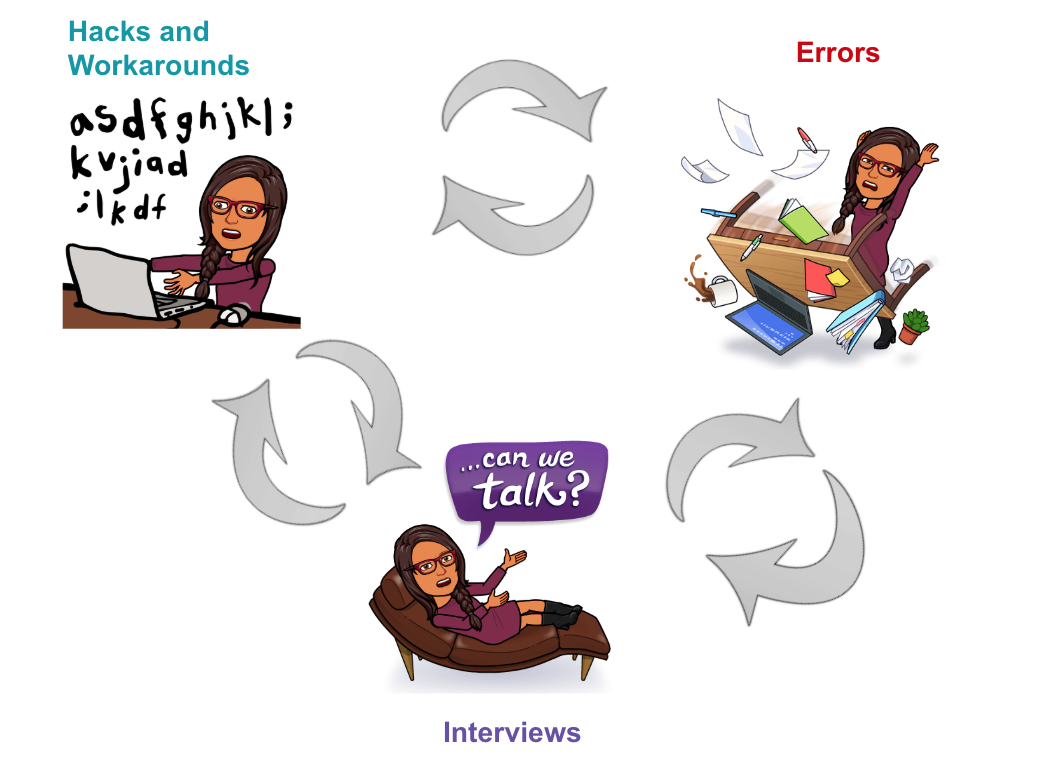
\includegraphics[scale=.5]{approach_cycle.png}
\caption{Needfinding approach cycle.}
\label{fig::7}
\end{figure}

\bibliographystyle{apacite} 
\bibliography{bibtemp}

\end{document}
